%%%%%%%%%%%%%%%%%%%%%%%%%%%%%%%%%%%%%%%%%
% Beamer Presentation
% LaTeX Template
% Version 1.0 (10/11/12)
%
% This template has been downloaded from:
% http://www.LaTeXTemplates.com
%
% License:
% CC BY-NC-SA 3.0 (http://creativecommons.org/licenses/by-nc-sa/3.0/)
%
%%%%%%%%%%%%%%%%%%%%%%%%%%%%%%%%%%%%%%%%%

%----------------------------------------------------------------------------------------
%	PACKAGES AND THEMES
%----------------------------------------------------------------------------------------

\documentclass{beamer}

\mode<presentation> {
	
	% The Beamer class comes with a number of default slide themes
	% which change the colors and layouts of slides. Below this is a list
	% of all the themes, uncomment each in turn to see what they look like.
	
	%\usetheme{default}
	%\usetheme{AnnArbor}
	%\usetheme{Antibes}
	%\usetheme{Bergen}
	%\usetheme{Berkeley}
	%\usetheme{Berlin}
	%\usetheme{Boadilla}
	%\usetheme{CambridgeUS}
	%\usetheme{Copenhagen}
	%\usetheme{Darmstadt}
	%\usetheme{Dresden}
	%\usetheme{Frankfurt}
	%\usetheme{Goettingen}
	%\usetheme{Hannover}
	%\usetheme{Ilmenau}
	%\usetheme{JuanLesPins}
	%\usetheme{Luebeck}
	\usetheme{Madrid}
	%\usetheme{Malmoe}
	%\usetheme{Marburg}
	%\usetheme{Montpellier}
	%\usetheme{PaloAlto}
	%\usetheme{Pittsburgh}
	%\usetheme{Rochester}
	%\usetheme{Singapore}
	%\usetheme{Szeged}
	%\usetheme{Warsaw}
	
	% As well as themes, the Beamer class has a number of color themes
	% for any slide theme. Uncomment each of these in turn to see how it
	% changes the colors of your current slide theme.
	
	%\usecolortheme{albatross}
	\usecolortheme{beaver}
	%\usecolortheme{beetle}
	%\usecolortheme{crane}
	%\usecolortheme{dolphin}
	%\usecolortheme{dove}
	%\usecolortheme{fly}
	%\usecolortheme{lily}
	%\usecolortheme{orchid}
	%\usecolortheme{rose}
	%\usecolortheme{seagull}
	%\usecolortheme{seahorse}
	%\usecolortheme{whale}
	%\usecolortheme{wolverine}
	
	%\setbeamertemplate{footline} % To remove the footer line in all slides uncomment this line
	%\setbeamertemplate{footline}[page number] % To replace the footer line in all slides with a simple slide count uncomment this line
	
	%\setbeamertemplate{navigation symbols}{} % To remove the navigation symbols from the bottom of all slides uncomment this line
}

\usepackage{graphicx} % Allows including images
\usepackage{subfigure}
\usepackage{booktabs} % Allows the use of \toprule, \midrule and \bottomrule in tables
\usepackage{bm}

%----------------------------------------------------------------------------------------
%	TITLE PAGE
%----------------------------------------------------------------------------------------

\title[Selective Inference]{Selective Inference for Hierarchical Clustering} % The short title appears at the bottom of every slide, the full title is only on the title page

\author{Ganchao Wei} % Your name
%\institute[UConn] % Your institution as it will appear on the bottom of every slide, may be shorthand to save space
%{
%University of Connecticut \\ % Your institution for the title page
%\medskip
%\textit{ganchao.wei@uconn.edu} % Your email address
%}
\date{October 6, 2021} % Date, can be changed to a custom date

\begin{document}
	
	\begin{frame}
		\titlepage % Print the title page as the first slide
	\end{frame}
	
	\begin{frame}
		\frametitle{Overview} % Table of contents slide, comment this block out to remove it
		\tableofcontents
	\end{frame}
	
	%--------------------------------------------------------------------
	%	PRESENTATION SLIDES
	%--------------------------------------------------------------------
	
	\section{Introduction and Motivation}
	
	\begin{frame}
		\frametitle{Introduction \& Motivation}
		\textbf{Goal}: Test for a difference in means between groups.\\
		But... The groups are usually defined via clustering $\Rightarrow$ inflate type I error if using the classical test.\\
		\textbf{Settings}: $\bm{X}\sim MN_{n\times q}(\bm{\mu}, \bm{I}_n, \sigma^2\bm{I}_q)$, where $\bm{\mu}$ and $\sigma^2>0$ is known.\\
		Define the population \& empirical row mean of $\mathcal{G}$ as $\bar{\mu}_{\mathcal{G}} = \frac{1}{|\mathcal{G}|}\sum_{i\in\mathcal{G}}\mu_i$ and $\bar{X}_{\mathcal{G}} = \frac{1}{|\mathcal{G}|}\sum_{i\in\mathcal{G}}X_i$\\
		\textbf{Test}: $H_0^{\{\hat{C}_1, \hat{C}_2\}}: \bar{\mu}_{\hat{C}_1} = \bar{\mu}_{\hat{C}_1}$ vs. $H_1^{\{\hat{C}_1, \hat{C}_2\}}: \bar{\mu}_{\hat{C}_1} \ne \bar{\mu}_{\hat{C}_1}$\\
		\textbf{Traditional Wald Test}: $\mathbb{P}_{H_0^{\{\hat{C}_1, \hat{C}_2\}}}(||\bar{X}_{\hat{C}_1} - \bar{X}_{\hat{C}_2}||_2 \geq ||\bar{x}_{\hat{C}_1} - \bar{x}_{\hat{C}_2}||_2)$, which can be calculated using $(\sigma\sqrt{\frac{1}{\hat{C}}_1 + \frac{1}{\hat{C}_2}})\cdot\chi_{q}$.\\
		This is problematic! Even when there's no signal, clustering is maximizing the differences between clusters. In other words, we use the data to select the null $\Rightarrow$ null distribution of the Wald test statistic is not proportional to a $\chi_{q}$ distribution $\Rightarrow$ too aggressive (inflate $\alpha$).
		
	\end{frame}
	
	%------------------------------------------------
	
	\begin{frame}
		\frametitle{Introduction \& Motivation}
		2000 simulated data: $\mathbf{\mu} = \mathbf{0}_{100\times2}$ and $\sigma^2 = 1$. Average linkage hierarchical clustering.
		\begin{figure}
			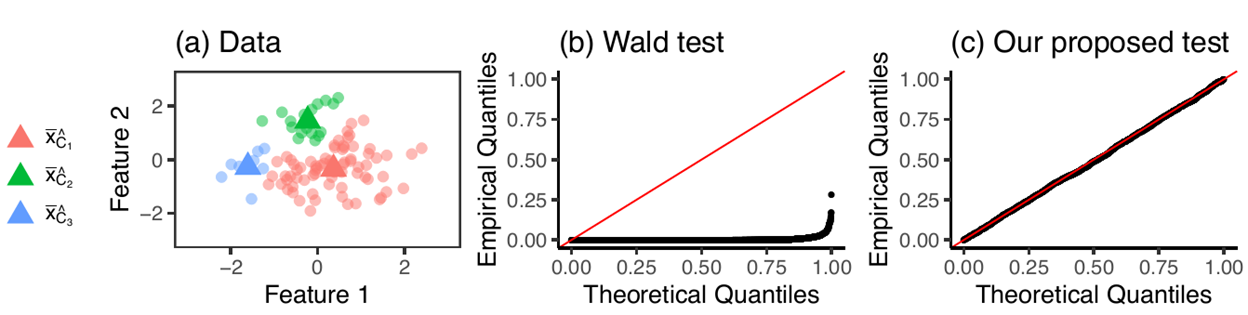
\includegraphics[width=0.7\linewidth]{image001.png}
		\end{figure}
		Maybe data splitting can remedy that? Do clustering in training set and then do 3-NN in test set.
		\begin{figure}
			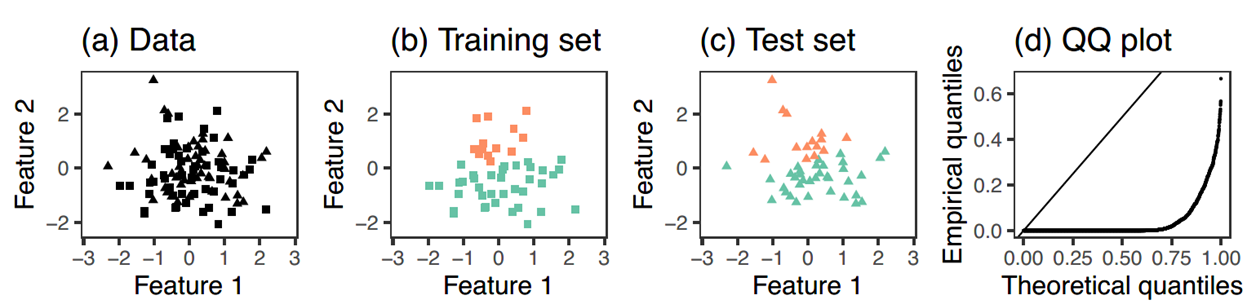
\includegraphics[width=0.7\linewidth]{image002.png}
		\end{figure}
		It still doesn't work...Use the data to select null hypothesis, and $H_0^{\{\hat{C}_1, \hat{C}_2\}}$ is a function of test observations.
	\end{frame}
	
	%------------------------------------------------
	\begin{frame}
		\frametitle{Introduction \& Motivation}
		In this paper, they develped a selective inference framework to test for a difference in means after clustering.\\
		\textbf{key idea}: define p-value that conditions on the event $\{\hat{C}_1, \hat{C}_2 \in C(\bm{X})\}$\\
		Compared to previous research:
		\begin{itemize}
			\item
			Don't need resampling \& provide exact finite-sample inference (if $\sigma$ is known).
			\item
			No need for sample splitting, and allows inference on all the data. 
		\end{itemize}
	\end{frame} 
	
	\section{Selective Inference for Clustering}
	
	%------------------------------------------------
	\begin{frame}
		\frametitle{Selective Inference: framework for test}
		\textbf{Conditional p-value}: $\mathbb{P}_{H_0^{\{\hat{C}_1, \hat{C}_2\}}}(||\bar{X}_{\hat{C}_1} - \bar{X}_{\hat{C}_2}||_2 \geq ||\bar{x}_{\hat{C}_1} - \bar{x}_{\hat{C}_2}||_2 | \hat{C}_1, \hat{C}_2 \in C(\bm{X}))$\\
		$H_0^{\{\hat{C}_1, \hat{C}_2\}}$ controls the \textbf{selective type I error rate for clustering} if $\mathbb{P}_{H_0^{\{\hat{C}_1, \hat{C}_2\}}}(reject \  H_0^{\{\hat{C}_1, \hat{C}_2\}} at\  level\ \alpha | \hat{C}_1, \hat{C}_2 \in C(\bm{X}))\leq \alpha$\\
		We can redefine the p-value as :
		\begin{figure}
			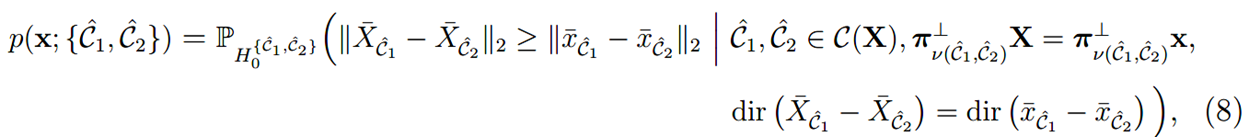
\includegraphics[width=1\linewidth]{image003.png}
		\end{figure}
		, where $\bm{\pi}^{\perp}_\nu$ projects onto the orthogonal complement of the vector $\nu$ and $\nu(\hat{C}_1, \hat{C}_2)_{i} = \bm{1} \{i\in\ \hat{C}_1\}|\hat{C}_1| - \bm{1}\{i\in\ \hat{C}_2\}|\hat{C}_2|$
		
	\end{frame}
	
	%------------------------------------------------
	\begin{frame}
		\frametitle{Selective Inference: framework for test}
		\begin{figure}
			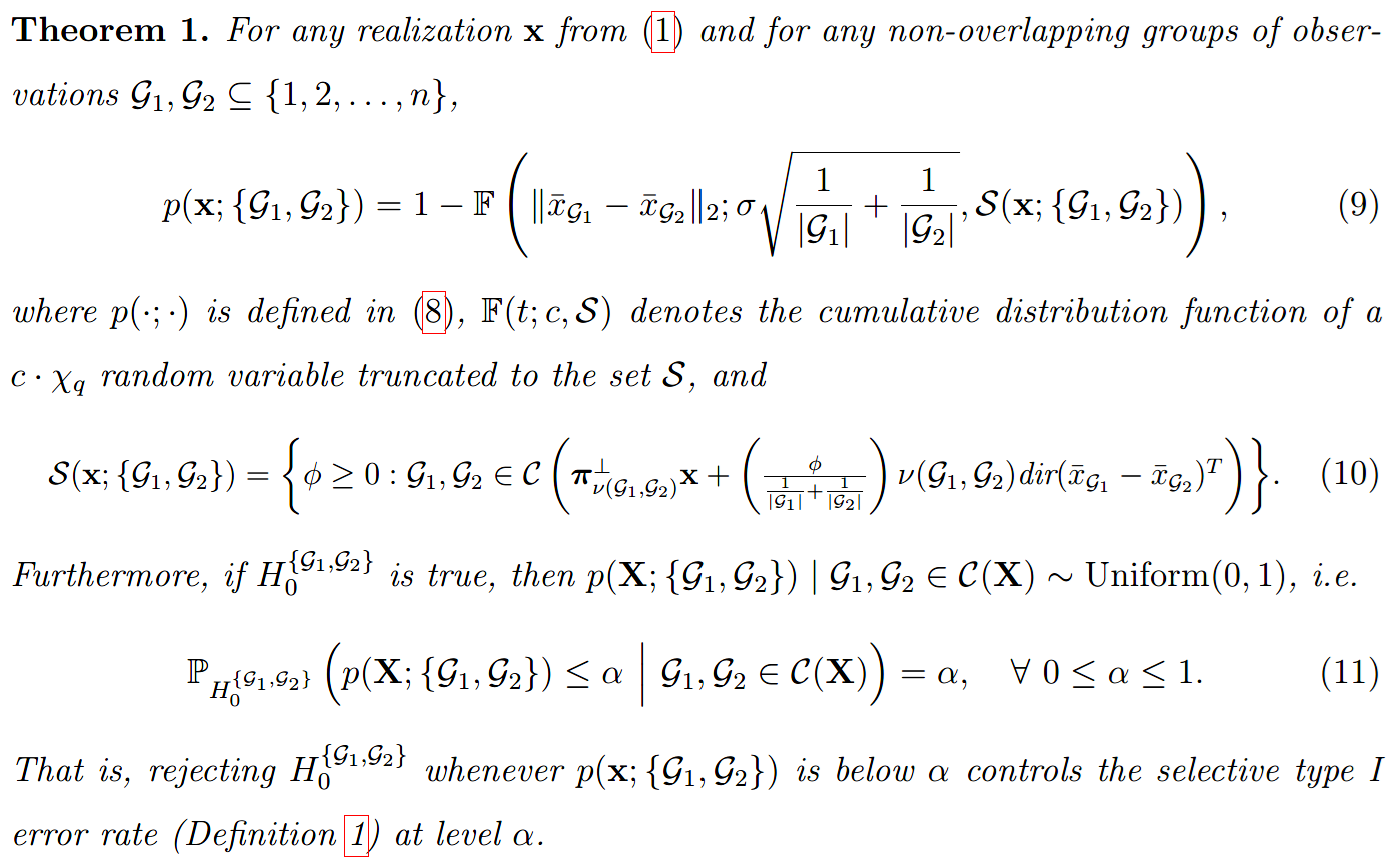
\includegraphics[width=1\linewidth]{image004.png}
		\end{figure}
	\end{frame}
	
	%------------------------------------------------
	\begin{frame}
		\frametitle{Selective Inference: framework for test}
	So, to compute p-value, it suffices to characterize $\hat{S}=S(\bm{x}; \{\hat{C}_1, \hat{C}_2\}) = \{\phi \geq 0: \hat{C}_1, \hat{C}_2 \in C(\bm{x}'(\phi))\}$, where 
	\begin{figure}
		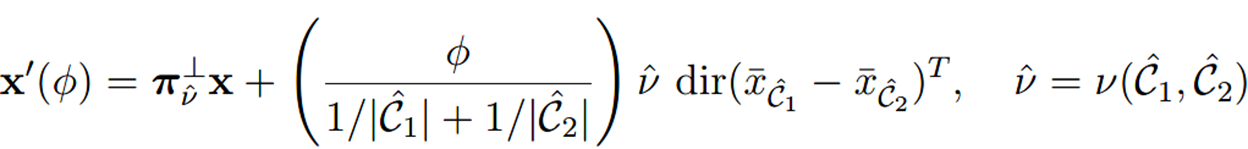
\includegraphics[width=.8\linewidth]{image009.png}
	\end{figure}
	Not very intuitive... Since $\bm{x}^{'}\hat{\nu} = \bar{x}_{\hat{C}_1} - \bar{x}_{\hat{C}_2}$, the $i$th row of $\bm{x}'(\phi)$ is:
	\begin{figure}
		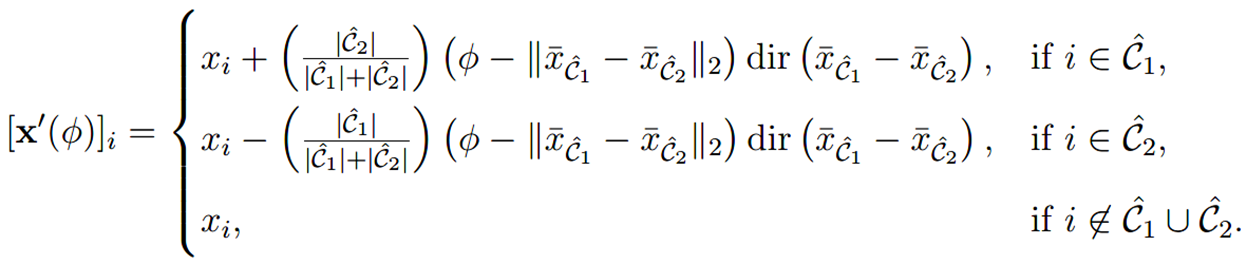
\includegraphics[width=.8\linewidth]{image010.png}
	\end{figure}
	So, that means observations in $\hat{C}_1 $ and $\hat{C}_2$ will:
	\begin{itemize}
		\item
		be pulled apart, if $\phi > ||\bar{x}_{\hat{C}_1} - \bar{x}_{\hat{C}_2}||_2$ .
		\item
		keep the unchanged, if $\phi = ||\bar{x}_{\hat{C}_1} - \bar{x}_{\hat{C}_2}||_2$
		\item
		be pushed together, if $0 \leq \phi < ||\bar{x}_{\hat{C}_1} - \bar{x}_{\hat{C}_2}||_2$
	\end{itemize}
	\end{frame}
	
	%------------------------------------------------
	\begin{frame}
		\frametitle{Selective Inference: framework for test}
		$\bm{x}'(\phi)$ = perturbed version of $\bm{x}: $observations in $\hat{C}_1 $ and $\hat{C}_2$ will
		\begin{itemize}
			\item
			be pulled apart, if $\phi > ||\bar{x}_{\hat{C}_1} - \bar{x}_{\hat{C}_2}||_2$ .
			\item
			keep the unchanged, if $\phi = ||\bar{x}_{\hat{C}_1} - \bar{x}_{\hat{C}_2}||_2$
			\item
			be pushed together, if $0 \leq \phi < ||\bar{x}_{\hat{C}_1} - \bar{x}_{\hat{C}_2}||_2$
		\end{itemize}
		\begin{figure}
			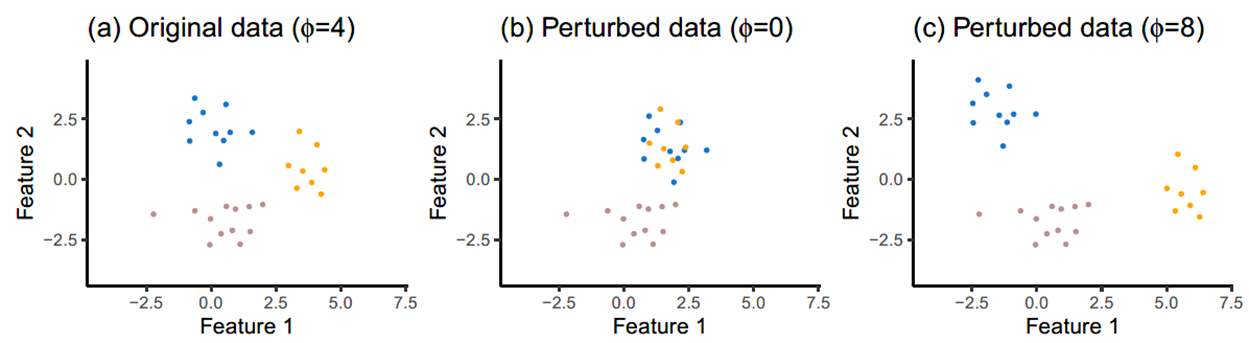
\includegraphics[width=1\linewidth]{image011.png}
		\end{figure}
	In (b), the algorithm no longer estimates these clusters. In this example, $\hat{S} = [2.8, \infty)$\\
	Furthermore, $\hat{S}$ describes the set of $\phi$, s.t. the algorithm preserves the results after perturbation.
	\end{frame}
	
	%------------------------------------------------
	\begin{frame}
		\frametitle{Computing $\hat{S}$ for hierachical clustering}
		By previous definition, we can simply calculate the p-value by Monte Carlo (later). But we can make use of properties in hierarchical clustering (e.g. dissimilarity \& linkage) to save computation time for $\hat{S}$.\\
		Let
		\begin{figure}
			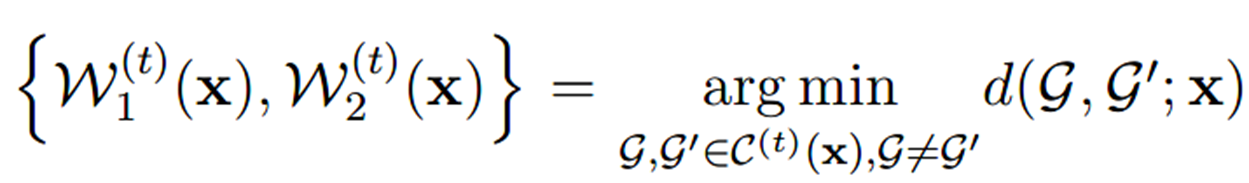
\includegraphics[width=.5\linewidth]{image012.png}
		\end{figure}
		be the 'winning pair' at step t. Then there's a Lemma about the height and merges, after perturbation (next page)
		
	\end{frame}
	
	%------------------------------------------------
	\begin{frame}
		\frametitle{Computing $\hat{S}$ for hierachical clustering}
		\begin{figure}
			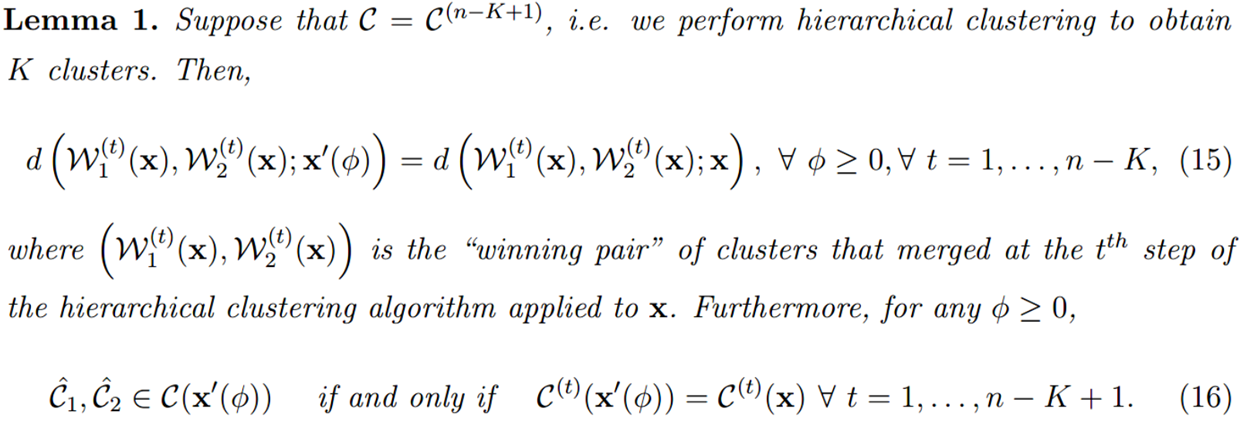
\includegraphics[width=1\linewidth]{image013.png}
		\end{figure}
		In short, the height and merges in the first $n-K$ steps keep the same after perturbation.
	\end{frame}
	
	%------------------------------------------------
	\begin{frame}
		\frametitle{Computing $\hat{S}$ for hierachical clustering}
		If we further define the "losing pairs" as:
		\begin{figure}
			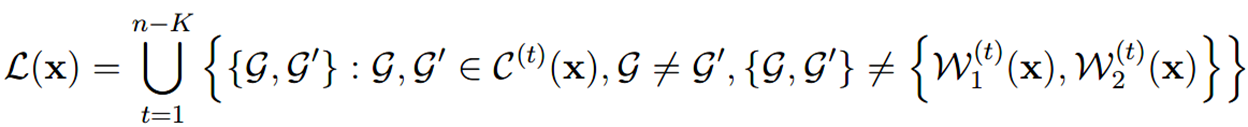
\includegraphics[width=1\linewidth]{image016.png}
		\end{figure}
		, and lower \& upper bound of life time:
		\begin{figure}
			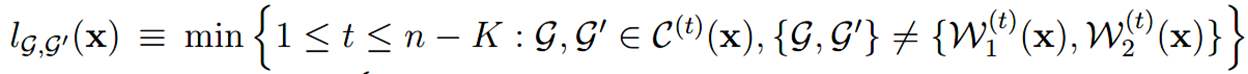
\includegraphics[width=1\linewidth]{image017.png}
			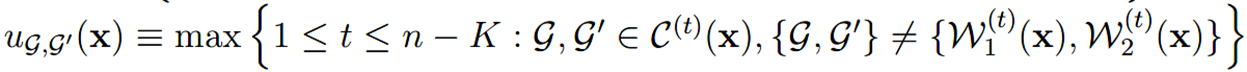
\includegraphics[width=1\linewidth]{image018.png}
		\end{figure}
		Then, we can calculate $\hat{S}$ as shown in the next page.
	\end{frame}
	
	%------------------------------------------------
	\begin{frame}
		\frametitle{Computing $\hat{S}$ for hierachical clustering}
		\begin{figure}
			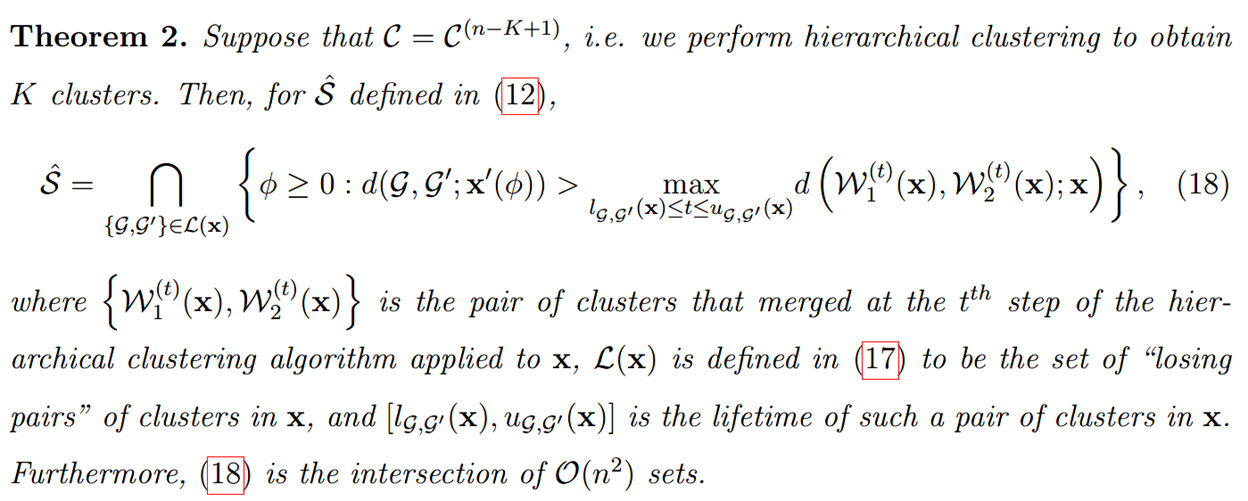
\includegraphics[width=1\linewidth]{image020.png}
		\end{figure}
	They further show details about when and how these sets can be efficiently computed.\\
	In particular, by specializing to squared Euclidean distance \& a certain class of linkages, each of these sets is defined by a single quadratic inequality and the coefficients can be efficiently computed.
	\end{frame}
	
	\section{Extensions}
	
	%------------------------------------------------
	\begin{frame}
		\frametitle{Extentions}
		\textbf{Extension 1}: Monte Carlo approximation to p-value\\
		The previous results only apply for hierarchical clustering, excluding the complete linkage. So we have to estimate p-value by Monte Carlo:
		\begin{figure}
			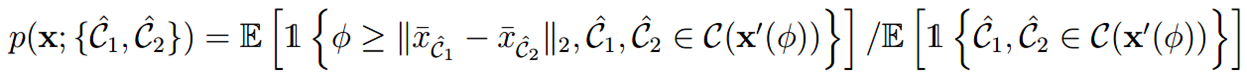
\includegraphics[width=1\linewidth]{image021.png}
		\end{figure}
		for $\phi\sim(\sqrt{\frac{1}{\hat{C}_1} + \frac{1}{\hat{C}_2}})\cdot\chi_{q}$\\
		To sample efficiently, we can further implement importance sampling.
		\textbf{Extension 2}: Non-spherical covariance matrix: 
		when $\bm{X}\sim MN_{n\times q}(\bm{\mu}, \bm{I}_n, \bm{\Sigma})$\\
		\textbf{Extension 3}: Unknown variance: 
		just plug in the estimate of $\sigma$.
	\end{frame}
	
	\section{Simulation}
	%------------------------------------------------
	\begin{frame}
		\frametitle{Simulation Results: Uniform p-values}
		$\bm{X}\sim MN_{n\times q}(\bm{\mu}, \bm{I}_n, \sigma^2\bm{I}_q)$, with $\bm{\mu} = \bm{0}_{n \times q}$\\
		Simulate 2000 data sets for $n = 150$, $\sigma \in \{1, 2, 10\}$ and $q \in \{2, 10, 100\}$
		\begin{figure}
			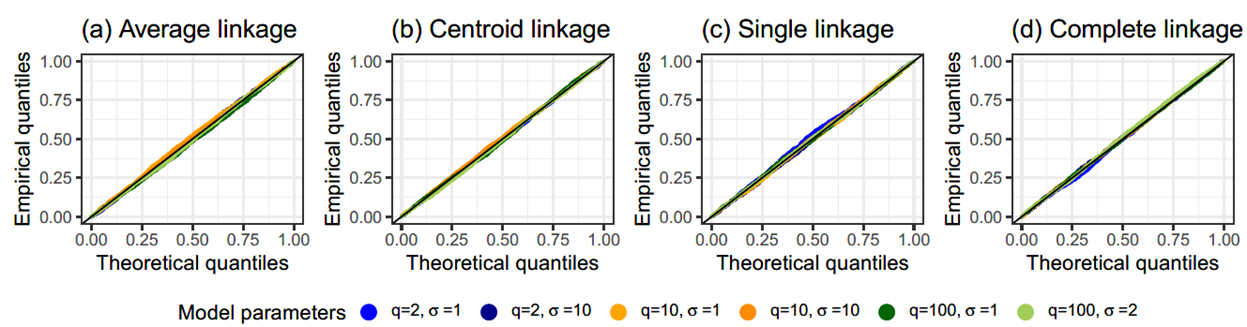
\includegraphics[width=1\linewidth]{image023.png}
		\end{figure}
	\end{frame}
	
	
	%------------------------------------------------
	\begin{frame}
		\frametitle{Conditional power and detection probability}
		They further check the conditional power and detection probability. Still under the setting $\bm{X}\sim MN_{n\times q}(\bm{\mu}, \bm{I}_n, \sigma^2\bm{I}_q)$, with $n = 30$. But now there are 3 equidistant clusters,
		\begin{figure}
			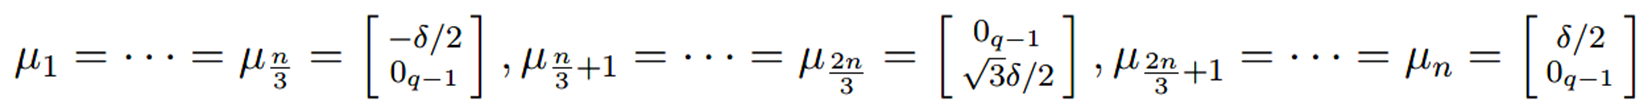
\includegraphics[width=1\linewidth]{image024.png}
		\end{figure}
		They simulated 300,000 dat sets for $\sigma=1$, $q = 10$ and 7 evenly-spaced values of $\delta\in [4,7]$. The significance level is $\alpha = 0.05$.
		The conditional power is defined as:
		\begin{figure}
			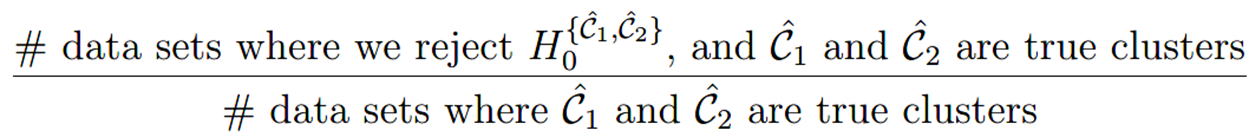
\includegraphics[width=.9\linewidth]{image025.png}
		\end{figure}
		The detection probability is defined as: 
		\begin{figure}
			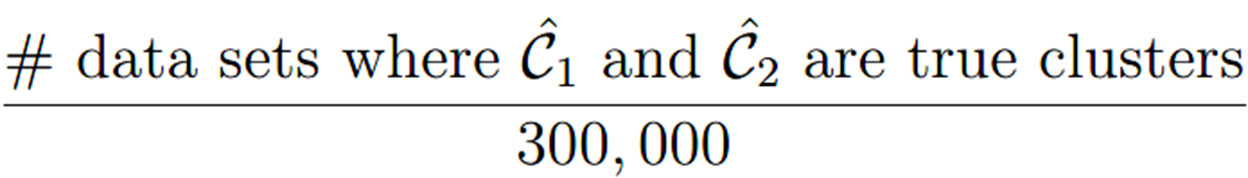
\includegraphics[width=.6\linewidth]{image026.png}
		\end{figure}
	\end{frame}
	
	
	%------------------------------------------------
	\begin{frame}
		\frametitle{Conditional power and detection probability}
		\begin{figure}
			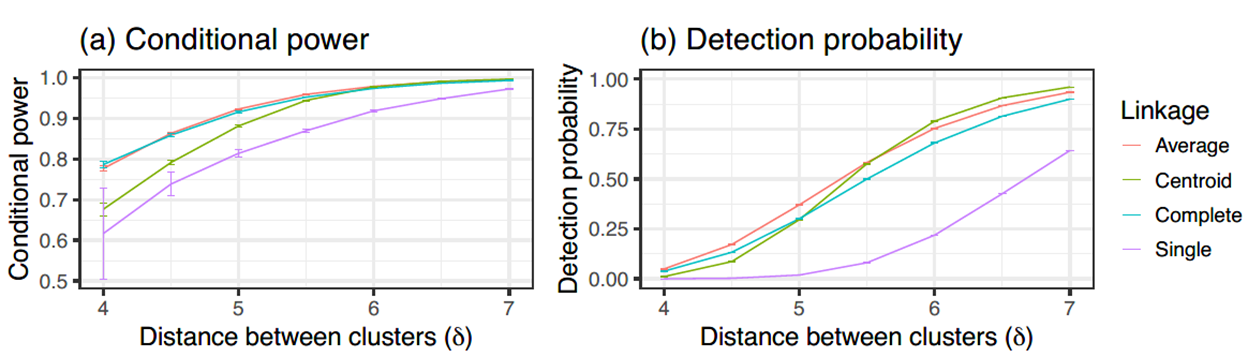
\includegraphics[width=1\linewidth]{image027.png}
		\end{figure}
		\begin{itemize}
			\item 
			conditional power and detection probability increases as distance between clusters increase
			\item
			Conditional power: average and complete linkage highest; single linkage lowest.
			\item
			Detection probabilities: average, centroid \& complete $\gg$ single
		\end{itemize}
	\end{frame}
	
	\section{Application}
	%------------------------------------------------
	\begin{frame}
		\frametitle{Application 1: Palmer penguins}
		First, estimate $\sigma$ from a separated data: bill length and flipper length of 58 female penguins in 2009.\\
		Then do average linkage hierarchical clustering with squared Euclidean distance to 107 penguins in 2007-2008. The features are still bill length and flipper length. 
		\begin{figure}
			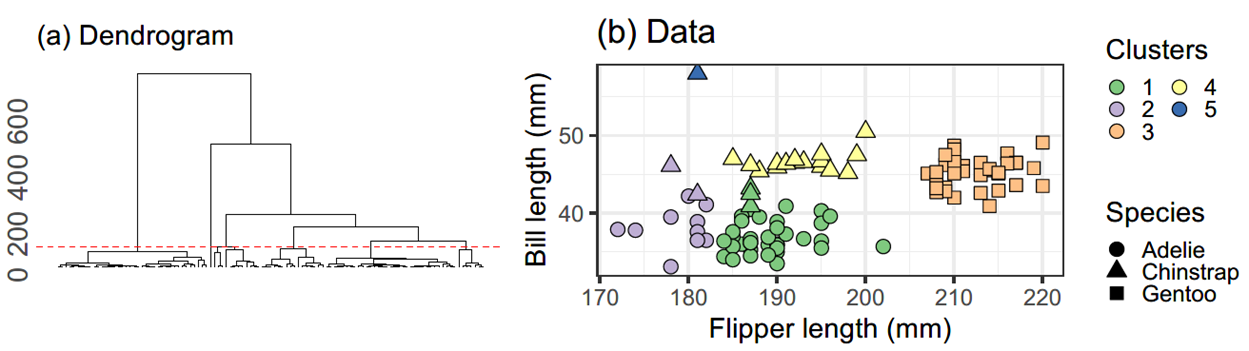
\includegraphics[width=.8\linewidth]{image028.png}
			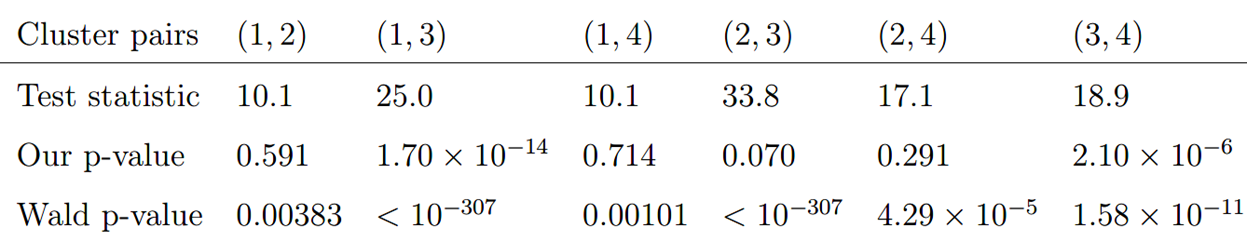
\includegraphics[width=.8\linewidth]{image029.png}
		\end{figure}
	\end{frame}
	
	
	%------------------------------------------------
	\begin{frame}
		\frametitle{Application 2: Single-cell RNA sequencing data}
		After pre-processing, there are 2 datasets (all with 500 genes):
		\begin{itemize}
			\item
			"no clusters": randomly sampling 600 memory T cells.
			\item
			"clusters": randomly sampling 200 each of memory T cells, B cells and monocytes. 
		\end{itemize}
		Apply ward-linkage hierarchical clustering with squared Euclidean distance to data. The $\bm{\Sigma}$ in $\bm{X}\sim MN_{n\times q}(\bm{\mu}, \bm{I}_n, \bm{\Sigma})$  is estimated by principal complement thresholding ('POET') to the left out data set:
		\begin{itemize}
			\item
			"no clusters": 3 pseudo-clusters, containing 64, 428 and 108 cells.
			\item
			"clusters": nearly recover the true clusters.
		\end{itemize}
		corrected p-values make sense:
		\begin{figure}
			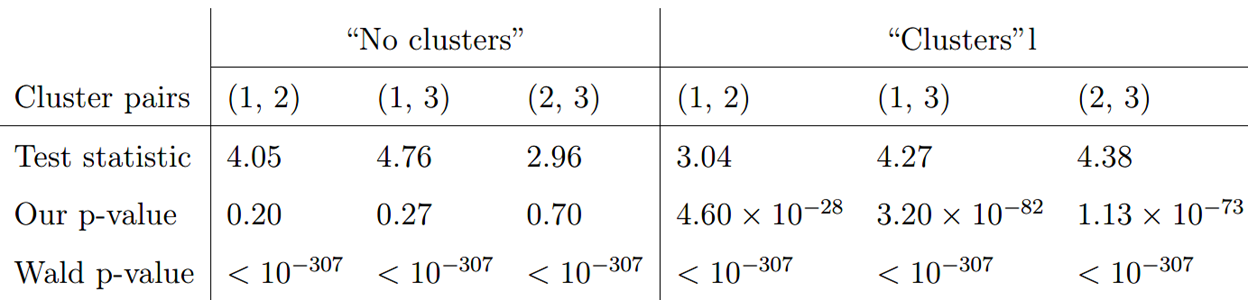
\includegraphics[width=.8\linewidth]{image031.png}
		\end{figure}
	\end{frame}
	
\end{document}